%Write why the Python in the next chapter.
%The core of the DO is the White Rabbit Trigger Distribution project, which allows the delivery of the timestamped events between %the devices. Internally, it uses the White Rabbit project for synchronisation and communication. In order to acquire and %imestamp the data, WR enabled digitizer board is used. At current state, only one board is supported ---FmcAdc100M14b4cha board %\cite{fmc_adc_ohwr}. In the future, support for other kinds of boards will be added. The DO itself is written in Python language, %using bindings to low level libraries. The technologies used in DO are presented in the following sections. 


%The idea of the DO is to allow to monitor the analog signals in the devices that could be located kilometers away from each other. In order to achieve this goal the DO uses the WRTD project, which allows distributing the triggers between the devices. The data is synchronised and sent to the final user. 


\chapter{Realisation of the DO}
The previous chapters describe the problem of the distributed data acquisition, the already existing solutions and how the DO approaches this problem and extends the previous concepts. In this chapter, the implementation of the DO is described in more detail.

For the implementation of the DO, the following work had to be done:
\begin{itemize}
    \item Deployment of the basic hardware setup, to demonstrate all of the crucial features of the system.
    \item Evaluation and selection of the most appropriate RPC.
    \item Implementation all the required applications:
    \begin{itemize}
        \item DO Server
        \item client applications:
        \begin{itemize}
            \item GUI
            \item test-bench
        \end{itemize}
        \item ADC application
    \end{itemize}
    \item Development of the design easy to test, debug and maintain afterwards.
    \item Development of the wrappers for the C libraries.
    \item Identification the issues of the WRTD.
    \item Optimisation the data transport.
    \item Optimisation the architecture.
\end{itemize}
All these issues are referred to in the following sections.

\section{Hardware setup and general concept} \label{section:hardware_setup}
    In order to demonstrate the crucial features of the DO, the setup presented in Fig.~\ref{fig:DO_hardware_setup}, Fig.~\ref{fig:DO_hardware_setup_photo} and Fig.~\ref{fig:DO_SPEC_FMC_front_panel} was deployed. The general concept of the DO is presented in Fig.~\ref{fig:DO_concept}.
    \begin{figure}
    	\centerline{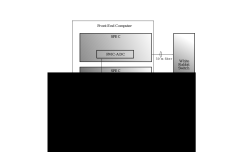
\includegraphics[width=\textwidth]{figures/DO_hardware_setup.pdf}}
    	\caption{The schematic of hardware setup of the DO}
    	\label{fig:DO_hardware_setup}
    \end{figure}
    \begin{figure}
    	\centerline{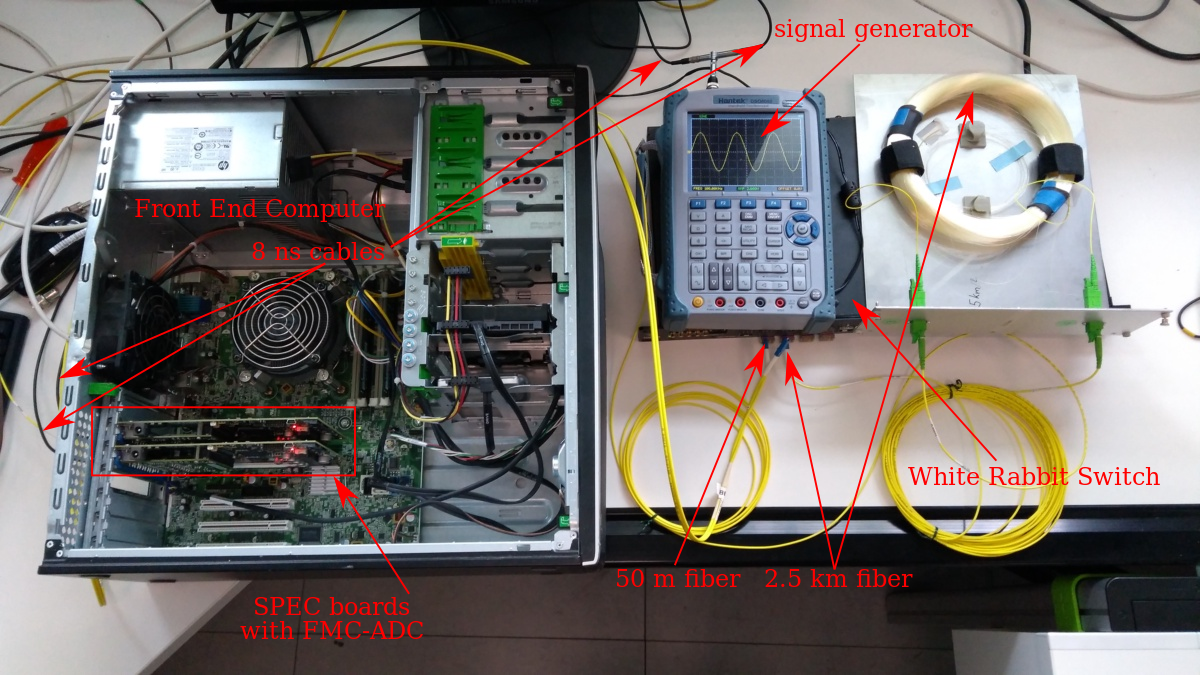
\includegraphics[width=\textwidth]{figures/DO_hardware_setup_photo.png}}
    	\caption{The photo of hardware setup of the DO}
    	\label{fig:DO_hardware_setup_photo}
    \end{figure}
    \begin{figure}
    	\centerline{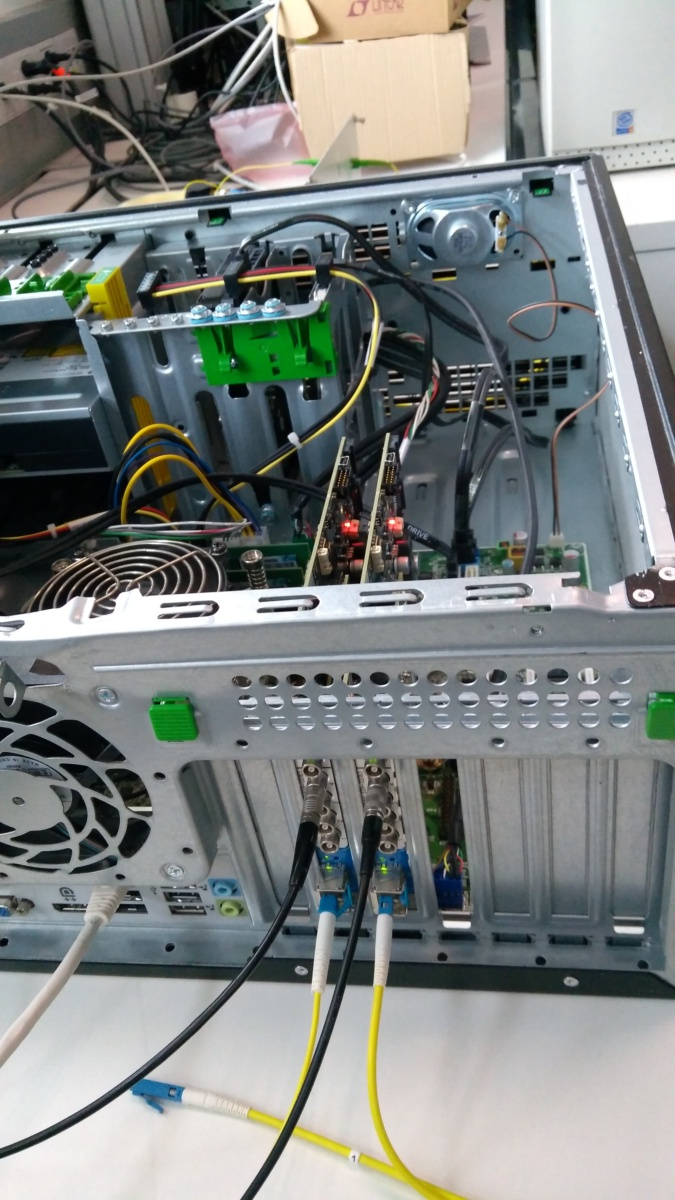
\includegraphics[width=0.6\textwidth]{figures/DO_SPEC_FMC_front_panel.jpg}}
    	\caption{The photo of the front panel of the SPEC board with FMC-ADC board}
    	\label{fig:DO_SPEC_FMC_front_panel}
    \end{figure}
    \begin{figure}
    	\centerline{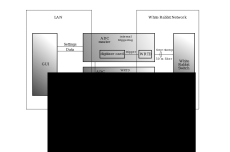
\includegraphics[width=\textwidth]{figures/DO_trigger_schem.pdf}}
    	\caption{The general concept of the DO}
    	\label{fig:DO_concept}
    \end{figure}
    
    In order to prove that the ADCs (section \ref{section:fmc_adc}) could acquire synchronised data independently of the distance, they were fed with the same sine signal and connected to the WR Switch (section \ref{section:WR}) with 50~m and 2.5~km fibres. Since both ADCs obtain exactly the same signal, measuring the phase shift between the obtained samples allows establishing the precision of the data synchronisation. Using fibre of a length in the range of kilometres allows simulating the synchronisation between the devices, whose distance is also in the range of kilometres. The schematic and photos depict the hardware setup and general conception of the DO. The software implementation details are presented in the next sections.


\section{RPC}   \label{section:rpc_selection}
    After implementation of the very first version of the DO and identification of the needs and the issues, the following list of requirements for the RPC was created:
    \begin{itemize}
        \item Transmission of synchronous messages --- this is the basic functionality of any RPC.
        \item Transmission of asynchronous messages --- it allows optimisation of the application.
        %\item Sending notifications --- in case at some point the communication scheme be changed and remove the publihser
        \item Polling on the connection --- it is common in many RPC libraries to create a separate thread for every connection. As described in section \ref{section:threads_management}, the DO is written with a minimum number of threads. For that reason, it was preferred to be able to poll on the connection and other file descriptors in the same thread, instead of adding new threads.
        \item Monitoring the state of the connection --- it allows detecting that the device was disconnected.
        \item It should use an efficient serialisation method or allow to serialise the data by an external library. It becomes important in case of sending large amounts of data. 
    \end{itemize}
    
    As the first approach, without yet having the requirements for the RPC, the XMLRPC was used. It was chosen mainly because it is very easy to deploy and it is in the Python Standard Library --- a smaller number of dependencies makes the project easier to maintain.
    After some time it was decided to look for another library because of the following reasons:
    \begin{itemize}
        \item It is not efficient. The reasons for the inefficiency are the following:
        \begin{itemize}
            \item It uses XML as the data format --- since it is a text format, unnecessarily big amounts of data are sent.
            \item It creates one connection per RPC instead of establishing a single communication channel.
        \end{itemize}
        \item It is impossible to send the dictionaries with integer keys: in the applications, the keys were converted into strings and then back to integers, only because of this restriction.
        \item It is impossible to send integers bigger than 24 bits --- bigger integers were split or converted to a string.
        \item It is not possible to monitor the state of the connection.
        \item Among all the previously mentioned requirements only two are satisfied, one of them partially:
        \begin{itemize}
            \item Transmission of synchronous messages.
            \item Polling on the connection --- it is possible only after modification of the source code of the XMLRPC server.
        \end{itemize}
    \end{itemize}
    
    After discovery of the problems with the XMLRPC, the previously mentioned list of the RPC requirements was created, to find the best solution. The following RPCs (described in section \ref{subsec:chap3:communication:rpc}) were taken into account:
    \begin{itemize}
        \item gRPC
        \item RPyC
        \item own implementation
    \end{itemize}
    
    None of the available libraries fulfils all the requirements. In the gRPC, it is impossible or difficult to monitor the state of the channel as well as there is no direct way to manually poll on the connection. In the RPyC there is no direct way to poll on the connection. 
    
    Finally, it was decided to use an own implementation of the RPC. It gives a lot of flexibility without or with very little of overhead in the development time. Most likely, if the custom implementation of the RPC was used straight away, it would have shortened the development time by avoiding the problems introduced by other libraries.
    
    %Choice of the transport
    It was decided to implement the RPC using ZeroMQ. The custom implementation of the RPC from now on will be called ZMQRPC. The other considered options were raw TCP sockets and another message queues. 
    
    %Why not TCP sockets
    The advantages of ZeroMQ sockets over raw TCP sockets are presented in section \ref{subsec:ZeroMQ}. The only advantage of the raw TCP sockets, in this case, is that it is easy to monitor the state of the TCP connection, while it is not the case for the ZeroMQ. The ZeroMQ provides an additional abstraction layer in order to provide reliable and robust transport of data, automatically reconnecting in case of lost connection. In many cases, it is desirable behaviour, but not in case of the DO. This problem could be overcome by adding timeouts when receiving the data from the sockets and implementing heart-beating. The heart-beating consists of periodically sending a message over the connection and in case of not receiving any reply for a predefined time, disconnecting the device. However, the heart-beating is not yet implemented in the DO.
    
    %Why not another message queues 
    Among other message queues libraries, the ZeroMQ was chosen based on the evaluation of various middle-ware products by the \textit{Software for Real-Time and Communication} group at CERN, presented in \cite{zmq_comparison} for the current equipment access framework \cite{zmq_icaleps}.
    
    The code for the basic RPC client is presented in Lis. \ref{cap:zmqrpc_client}
    
    \begin{lstlisting}[language=Python, 
                   caption = The code for basic RPC using ZeroMQ., 
                   label=cap:zmqrpc_client]
class ZMQ_RPC():                                                               
    def __init__(self, ip, port):                                              
        context = zmq.Context()                                                
        self.socket = context.socket(zmq.DEALER)                               
        self.socket.setsockopt(zmq.RCVTIMEO, 3000)                             
        addr = str(ip) + ':' + str(port)                                       
        self.socket.connect("tcp://" + addr)                                   
                                                                               
    def send_RPC(self, function_name, *args):                                  
        msg = [function_name, *args]                                           
        msg = pickle.dumps(msg)                                                
        self.socket.send(msg)                                                  
        try:                                                                   
            message = self.socket.recv()                                       
        except ZMQ_Timeout:                                                    
            logger.error("Server not replying")                                
            raise RPC_Error("Timeout of zmq socket.recv()")                    
            return None                                                        
        if message == b'Error':                                                
            logger.error(function_name + ' not available in the server')        
        else:                                                                  
            ret = pickle.loads(message)                                        
            logger.info(function_name + ' success')                            
            return ret  
\end{lstlisting}

    
    During the initialisation of the RPC client, the ZeroMQ socket is created, with a timeout equal to 3~s. The value of 3~s was selected in order not to block the program for too long in case of an error and not to be too short in case of any delay in the communication channel. In case of sockets where a delay in the communication channel is not expected, the value of the timeout is reduced. The socket connects to the server whose IP and port are provided. 
    
    The function responsible for executing the RPC, \textit{send\_RPC}, serialises the data, sends it through the socket and waits for the response. The response is returned to the caller.  
    
    The comparison of the XMLRPC server and ZMQRPC server is presented in Lis. \ref{cap:xmlrpc_server} and Lis. \ref{cap:zmqrpc_server} respectively. The code is practically the same. It consists of creation of a selector, registration of the server and polling on the file descriptor in the loop. Every time the poll returns, the call is executed.
    
    The reason for presenting these codes is to prove that custom implementation of the RPC does not introduce any overhead in the development time and is equally easy as using external library, giving at the same time more flexibility.
    
    \begin{lstlisting}[language=Python, 
                   caption = Examples code for XMLRPC server., 
                   label=cap:xmlrpc_server]
def run(self):    
    _ServerSelector = selectors.PollSelector                                   
    try:                                                                       
        with _ServerSelector() as selector:                                    
            selector.register(serv_expose.server, selectors.EVENT_READ)        
                                                                               
            while True:                                                        
                ready = selector.select(0.5)                                   
                if ready:                                                      
                    serv_expose.server._handle_request_noblock()               
                                                                               
                serv_expose.server.service_actions()                           
    finally:                                                                   
        pass 


\end{lstlisting}

    \begin{lstlisting}[language=Python, 
                   caption = Examples code for ZMQRPC server., 
                   label=cap:zmqrpc_server]
def run(self):                                                                 
    context = zmq.Context()                                                    
    socket = context.socket(zmq.ROUTER)                                        
    server_ip = get_ip()                                                       
    socket.bind("tcp://" + server_ip  + ":8003")                               
    poller = zmq.Poller()                                                      
    poller.register(socket, zmq.POLLIN | zmq.POLLERR)                          
                                                                               
    while True:                                                                
        socks = dict(poller.poll())                                            
        if socket in socks:                                                    
            [identity, message] = socket.recv_multipart()                      
            message = pickle.loads(message)                                    
            try:                                                               
                func = getattr(self, message[0])                               
                ret = func(*message[1:])                                       
                ret = pickle.dumps(ret)                                        
                socket.send_multipart([identity, ret])                         
            except AttributeError:                                             
                socket.send_multipart([identity, b"Error"]) 
\end{lstlisting}


    
    
\section{DO components} \label{section:do_components}

    \subsection{DO Server} \label{section:do_server_app}
        The DO Server is the central unit of the DO, responsible for management of the connections and for simple processing of data. 
        The simplified Unified Modeling Language (UML) class diagram of the DO Server application is presented in Fig.~\ref{fig:uml_server}.
        
        \begin{figure}
        	\centerline{\includegraphics[width=\textwidth]{figures/UML_server.pdf}}
        	\caption{Simplified UML class diagram of the DO Server application}
        	\label{fig:uml_server}
        \end{figure}
        
        The DO Server consists of four major components:
        \begin{itemize}
            \item User class --- it is a model of the User application. In principle it is independent of the application, should it be GUI, test-bench or any other kind. It stands true under the assumption that each of the User applications behaves similarly to the classic oscilloscope, that is, it allows to connect the channels, select the trigger and collect the data. In case of any special requirements, more specified classes could inherit from the User class. Until now it was not necessary.
            \item ADC class --- it is a model of the connected device composed from the classes that represent particular functionalities of the ADC:
            \begin{itemize}
                \item Channel
                \item Trigger
                \begin{itemize}
                    \item Internal Trigger
                    \item External Trigger
                \end{itemize}
                \item Acquisition Configuration
            \end{itemize}
            %In the future, the models of the FDs and TDCs are going to be added.
            \item Connection Manager class --- it is responsible for registration and unregistration of the users and the devices as well as for providing the access to them for other classes.
        
            \item Communication --- in the DO Server there are four kinds of sockets used for communication with other applications:
            \begin{itemize}
                \item RPC client --- sends the RPC requests and receives the returned value.
                \item RPC server --- listens for the RPC requests, calls the respective function and sends back the returned value.
                \item Publisher --- sends the data without waiting for the reply.
                \item Subscriber --- receives the asynchronous data.
            \end{itemize}
            The sockets that are used to send data/requests, that is \textit{User publisher} and \textit{ADC RPC client}, are private to respective classes. The sockets that have to listen to asynchronous data, that is \textit{ADC subscriber}, \textit{User RPC Server} and \textit{Zeroconf Subscriber} are private to the \textit{Expose class}, that passes the data/requests to the \textit{Connection Manager} or to the respective \textit{Users} or \textit{ADCs}. The \textit{Expose class} implements a polling loop to listen on all of its sockets.
        \end{itemize}
        
        The following section describes the standard operation of the DO Server and its interactions with other applications.
        
        %Behaviour
        \subsubsection{Normal operation}
            The normal operation of the DO Server consists of five elements:
            \begin{itemize}
                \item Connections management --- The \textit{Expose} class listens for commands from Users applications, Device applications and Zeroconf to add or remove a service. Whenever the command is received, it is passed to the \textit{Connection Manager}, which creates or deletes respective User or ADC objects. In case of connecting or disconnecting the ADC, the notification is sent to the User that the device is available or unavailable. 
                
                \item User modification --- the User application can request to connect:
                \begin{itemize}
                    \item to the channel --- the User can connect to the channels of any of the ADCs that are not used by another User.
                    \item trigger --- the user can select either to trigger on the dedicated trigger input of any of the available ADCs or on the threshold of one of the connected channels. Only one trigger source can be selected. Whenever the trigger is selected, the master's configuration is assigned to the corresponding ADC and slave's configuration is assigned to the rest of the ADCs used by the particular user (see section~\ref{section:data_synchronisation}). The WRTD is configured to receive the timestamps from the master ADC and to distribute them to the slave ADCs. The slave ADCs are configured to trigger on the respective WRTD events.
                \end{itemize}
                
                \item ADC modification --- when the User application wants to modify the ADC configuration, it sends a message to the DO Server. The message contains the name of the ADC together with the name and the value of the parameter to configure. The request is pre-processed and respective commands are sent to the ADC application. Since the ADC application accesses the real hardware, in order to make sure that there was no error during the hardware access, the configuration of the ADC is retrieved after each request to modify any of the parameters. 
                
                \item Acquisition --- just like in a normal oscilloscope there are two acquisition modes:
                \begin{itemize}
                    \item single --- in this mode the acquisition of the ADC is configured once. When available, the data is received from the ADC application and sent to the User application. 
                    \item run --- in this mode the acquisition is configured in the loop, in order to obtain the data continuously. The detailed description of the acquisition loop is described in section \ref{section:acquisition_loop_opt}
                \end{itemize}
            \end{itemize}
            
    \subsection{GUI} \label{section:do_gui_app}
        %goal
        The GUI provides easy remote access to the connected devices in order to modify their configurations, collect the data and display it. 
        
        %first approach
        In the first approach to design the GUI, all possible configurations of the ADCs were exposed. A screenshot of the application with two ADCs connected is presented in Fig. \ref{fig:gui_first_approach}.

        \begin{sidewaysfigure}
        	\centerline{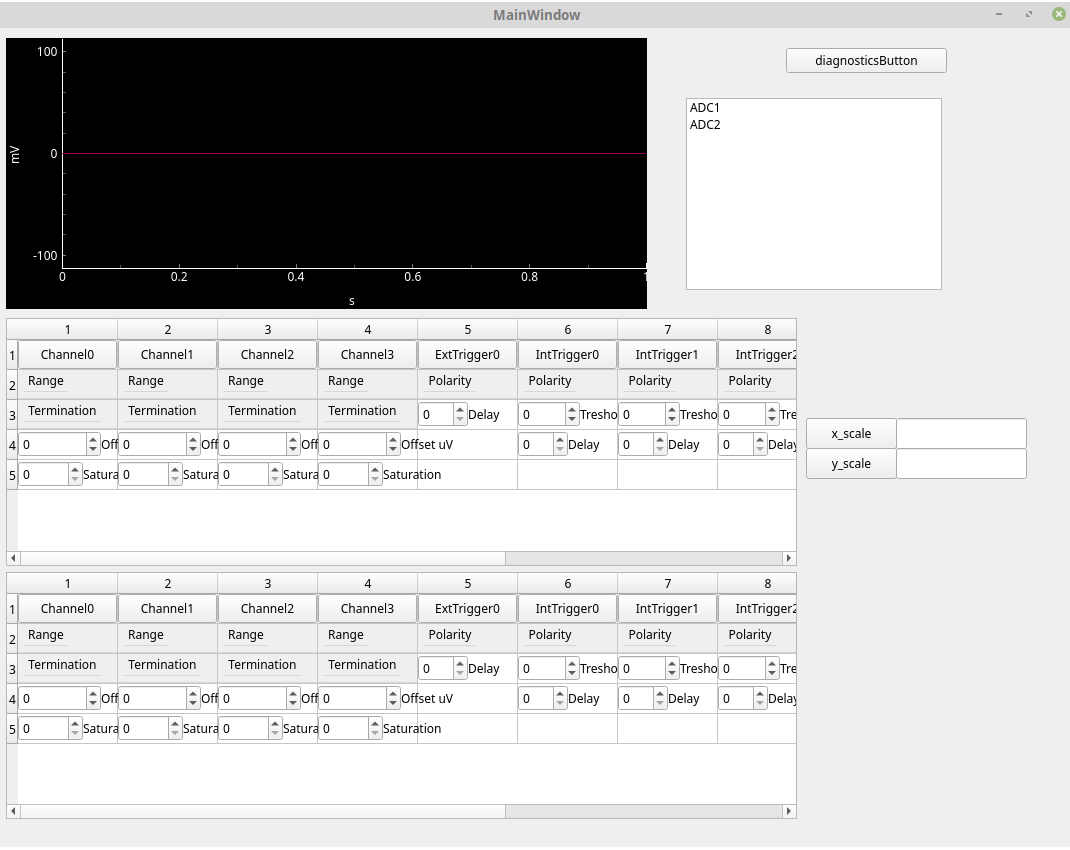
\includegraphics[width=0.9\textwidth]{figures/GUI_first_approach.jpg}}
        	\caption{The first version of the GUI}
        	\label{fig:gui_first_approach}
        \end{sidewaysfigure}
        
        It was a good starting point, which allowed to easily debug all the applications, but it turned out that in this way managing the synchronisation of the boards was more difficult. In order to configure the WRTD, the proper configuration of the triggers is necessary. Therefore there were two options:
        \begin{itemize}
            \item Allow the user to configure all the triggers.
            \item Hide some of the functionalities.
        \end{itemize}
        %why second approcah
        Since from the beginning of the project it was assumed that the synchronisation details should be hidden from the user, the second option was chosen. The updated version of the GUI is presented in Fig. \ref{fig:gui_current}.
        
        \begin{sidewaysfigure}
        	\centerline{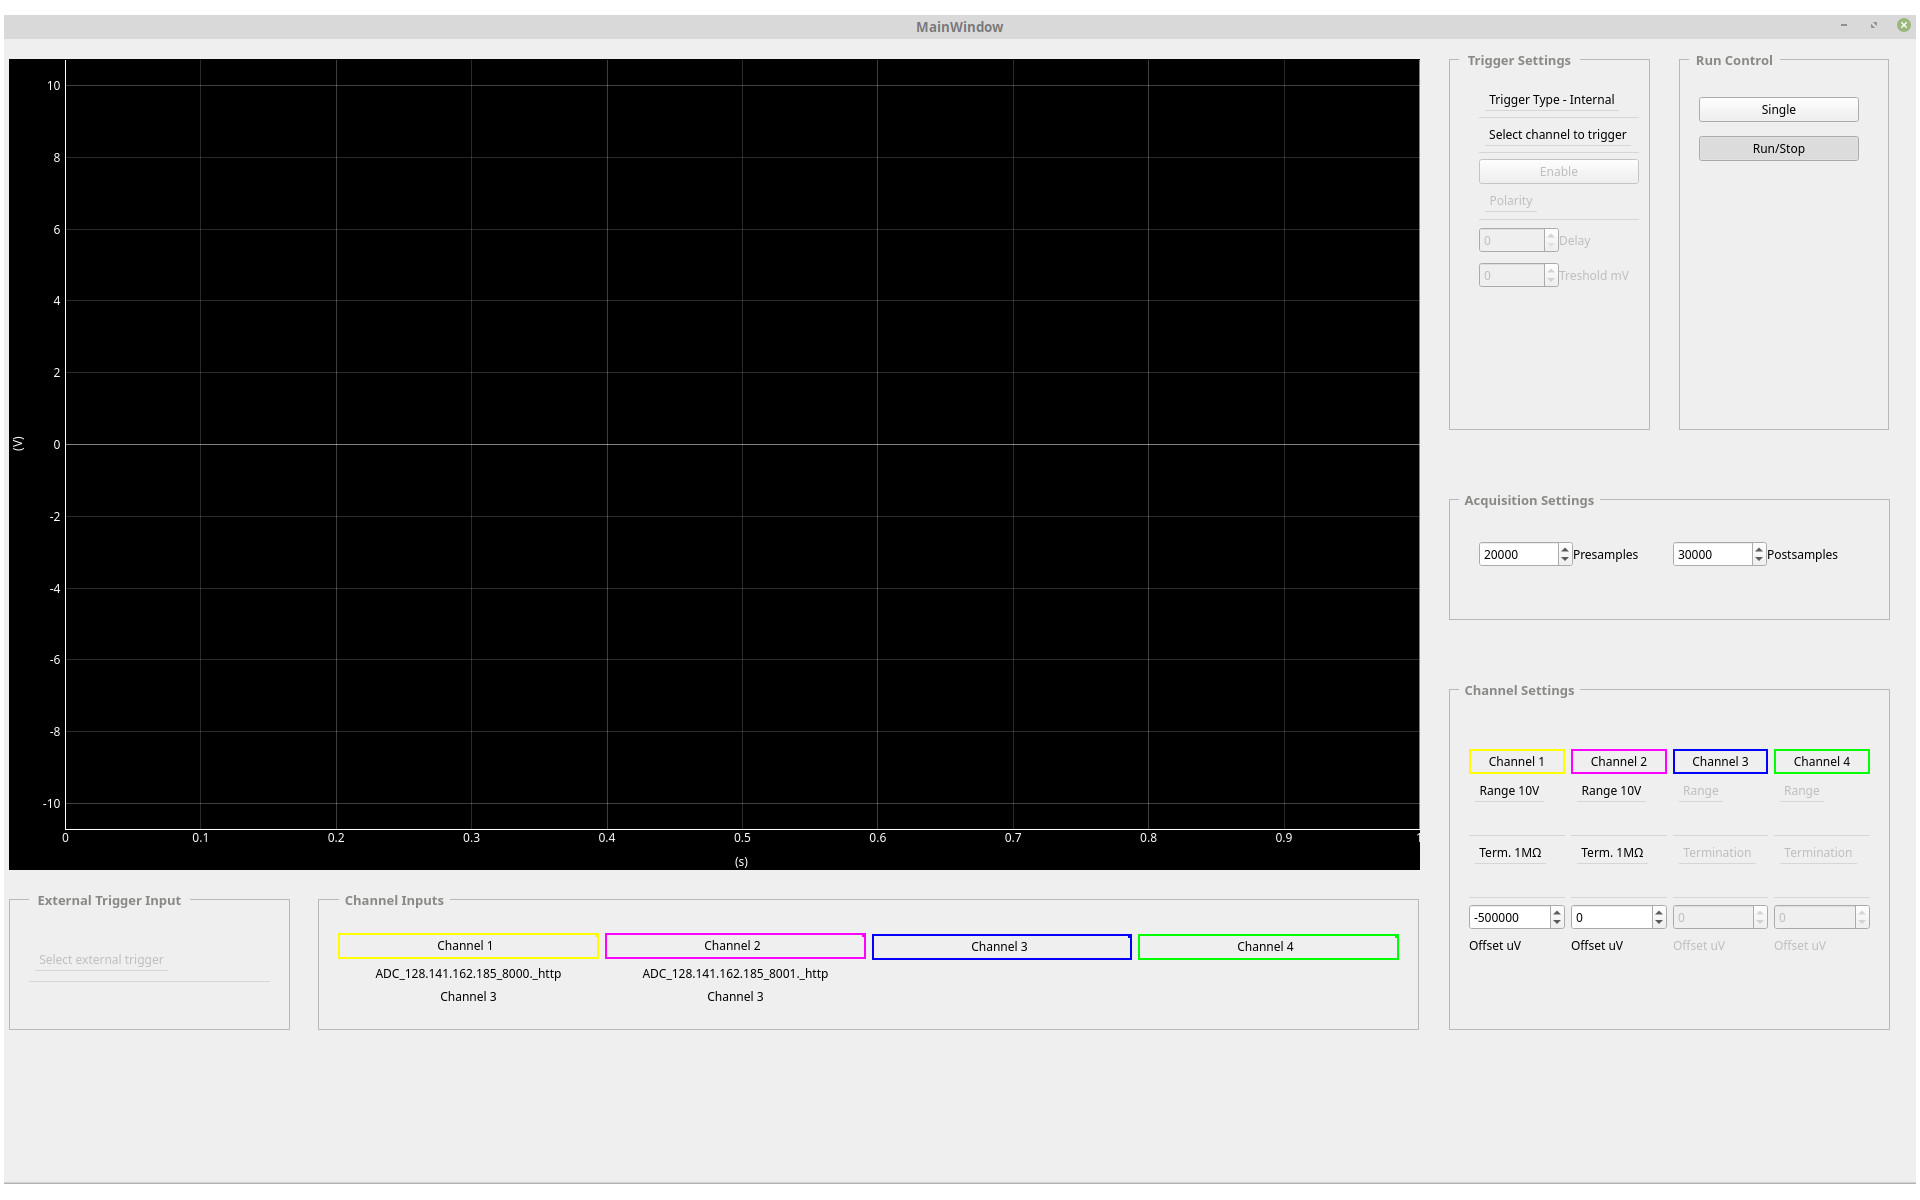
\includegraphics[width=\textwidth]{figures/GUI_current.jpg}}
        	\caption{The current version of the GUI}
        	\label{fig:gui_current}
        \end{sidewaysfigure}
        
        The design of the GUI was made as similar to the classical oscilloscope as possible. A special effort was made to make it intuitive, so that every electronics engineer could start using it just like every other oscilloscope.
        By now, it seems that this goal has been achieved partially. Taking into account the fact that the DO inevitably differs from a classical oscilloscope and there was not enough time to implement all the features of an oscilloscope, usually, some amount of explanation is needed for every new user.
        
        %design of the GUI
        Taking into account the chosen architecture (see section \ref{section:general_architecture}), it was assumed that the GUI should not process the data if it is not necessary and should only serve the three following functionalities:
        \begin{itemize}
            \item Allow the modification of the ADCs' parameters.
            \item Display the configuration of the ADCs.
            \item Display the acquired data.
        \end{itemize}
        The structure of the GUI application, presented in Fig. \ref{fig:gui_structure}, is straightforward. It is composed of various groups of settings of the oscilloscope and of the plot. Each group is composed of Qt widgets that have two functions:
        \begin{itemize}
            \item They represent the state of the setting they refer to.
            \item When the user modifies the widget, e.g. clicks on it, changes the value of the box etc., the widget invokes the function that is bound to it. The bound function, in the majority of cases, sends the information to the DO Server about the change of its state, using the RPC.
        \end{itemize}
        
        The \textit{server expose} module implements a polling loop to listen for the acquisition data and notifications about availability of the ADCs. Whenever any event is received, it uses the \textit{QT signals and slots mechanism} to transmit the data to the GUI.
        
        \begin{figure}
        	\centerline{\includegraphics[width=0.7\textwidth]{figures/GUI_schematics.pdf}}
        	\caption{Simplified GUI application diagram}
        	\label{fig:gui_structure}
        \end{figure}
    
    \subsection{ADC} \label{section:do_adc_app}
        The structure of the ADC application is presented in Fig. \ref{fig:adc_structure}.
        \begin{figure}
        	\centerline{\includegraphics[width=0.9\textwidth]{figures/ADC_schematics.pdf}}
        	\caption{Simplified ADC application diagram}
            	\label{fig:adc_structure}
        \end{figure}
        
        The purpose of the ADC application is to allow to remotely access the hardware resources:
        \begin{itemize}
            \item the ADC board
            \item the WRTD module
        \end{itemize}
        
        The ADC and the WRTD modules have full access to all of the hardware functionalities. However, for the purpose of the DO, direct access to the following functionalities is hidden:
        \begin{itemize}
            \item All of the WRTD functionalities.
            \item Pre-samples and post-samples modification --- the DO Server can select the value of the pre-samples and post-samples that it wants to receive, which does not always reflect the actual value used by the hardware (see section~\ref{section:data_synchronisation}).
        \end{itemize}
        The DO Server can select if the particular ADC works as the master or the slave in the network (see section~\ref{section:data_synchronisation}). With that information, the Device Access module appropriately configures the number of pre-samples and post-samples as well as it enables/disables necessary WRTD rules. 
        The rest of the ADC functionalities is exposed to the DO Server:
        \begin{itemize}
            \item Configuration of the ADC parameters.
            \item Retrieval of the configuration.
            \item Start/stop of the acquisition.
        \end{itemize}
        The communication with the DO Server is provided by the following modules:
        \begin{itemize}
            \item Zeroconf --- if the address of the DO Server is not known, Zeroconf notifies the DO Server about the presence of the new device.
            \item Publisher --- it publishes the acquired data. If the server address is known, it sends a notification about the presence of the new device to the DO Server.
            \item RPC server --- it provides remote access to the functionalities exposed by the Device Access. 
        \end{itemize}
        
        The libraries used to access the ADC board and the WRTD are written in C language. In order to ease the integration of the devices in the DO, Python wrappers were developed for both of these libraries. In order to directly access the C functions, the Python ctypes \cite{ctypes} library was used. The wrappers provide access to most of the functions provided by the libraries, except for the functions responsible for memory management, which is done automatically using Pythons constructors and destructors. The C specific parts of the library are hidden from the user.

    \subsection{Test-bench} \label{section:do_testbench_app}
        In order to provide a high quality code, a set of tests was developed.
        
        The most crucial elements of the DO are located in the DO Server and the ADC application. The GUI is responsible mainly to display the data and send the configuration. Therefore, taking into account the difficulty of writing the tests for graphical interfaces, it was decided to provide a script for testing the DO Server and the ADC. The features of the GUI are tested manually.
        
        The test script, which makes use of the Python unittest framework \cite{python_unittest}, replaces the GUI. Since the interface of the DO Server is generic, it is possible to connect various types of applications, including test-benches.
        
        The test script starts the DO Server application and the ADC applications. When the system is set, the test-bench connects to the DO Server as the User. Next, it sends the commands, reads back the configuration and compares if the data is coherent. Moreover, it provides the functionalities of measuring the acquisition time and frequency as well as the precision of the synchronisation. These functionalities were used to perform the measurements for this thesis.

\section{Threads management} \label{section:threads_management}
    The multi-threaded applications are desirable in case of systems that should be easily scalable. In a well-designed multi-threaded application, the processing capability increases with the number of processor cores. The main restriction that has to be taken into account is that the threads shouldn't access the same resources \cite{zeromq_guide}.
    
    The Python threads are not executed on different CPUs, so the code is not executed truly in parallel. These threads are generally used in cases when the code execution involves some waiting. That's why it seemed quite natural to use it for communication and data acquisition in the DO. During the development of the project, it was decided to minimise the number of threads because of the following reasons:
    \begin{itemize}
        \item The objects cannot be shared between the threads.
        \item To establish communication between the threads, the message queues have to be implemented. The functions that receive the data from the message queues are blocking, so adding such thread adds another level of abstraction without eliminating the problem.
        \item It is more difficult to debug the multi-threaded application.
        \item In case of wrong usage of mutexes it is easy to block the execution of the program.
    \end{itemize}
    
    If the execution of the program requires waiting for some resources, the alternative for using multiple threads is to use a single thread to poll on all of the resources in the loop and serve all of the requests. It avoids the problem of concurrent accesses and is much easier to debug. This approach is used in DO. However, additional threads were created in three cases:
    \begin{itemize}
        \item The GUI is run in the main thread, which is blocked after the start of the graphical interface. In order to receive the asynchronous data from the DO Server, using the non-QT library, it was necessary to implement a polling loop in the separate thread. The communication between the threads makes use of the \textit{QT signals and slots mechanism} \cite{qt_signals_slots}.
        \item The zeroconf service browser --- it uses one thread to listen for connections. Probably it would be possible to modify the code to poll on the file descriptor, but since it is a module with a very specific task, without any influence on the performance, it was decided to implement the message queue between the threads. For that purpose, the inter-process sockets are used.
        \item The test code starts the applications in different threads and uses the message queue to collect data from them.
    \end{itemize}
    The minimisation of the number of threads made the design much easier to test, debug and maintain afterwards.

\section{WRTD issues} \label{section:wrtd_issues}
The DO was the first user of the WRTD project before the release. One of the goals of the DO was to help to identify the issues of the WRTD before the release. Indeed, during the development of the project, the following issues were identified:
\begin{itemize}
    \item Single start of the acquisition was causing continuous acquisitions and flooding of the network with the timestamps.
    \item The timestamps were sent after the acquisition, not after receiving the trigger, which was causing the necessity of increasing the timestamp delay when increasing the number of acquired post-samples.
    \item Common bugs in the drivers and libraries of the ADC and WRTD --- eg. overflow etc.
    \item Wrong timing constraints of the HDL design that were causing communication errors.
    \item Issues with the ADC calibration.
    \item Issues with the acquisition of large numbers of samples.
\end{itemize}

Fast identification of the issues led to improvement of the tools.

    
\section{Acquisition speed optimisation} \label{section:acquisition_speed_optimisation}
    The amount of data that could be analysed in the distributed system depends on the acquisition frequency.
    In case of collecting data by the GUI in order to display it to the user, there is no point in increasing the frequency above what could be perceived by the human eye. 
    However, the data, instead of being plotted in the GUI, could be analysed to extract some information. In that case, there is no threshold frequency above which increasing it doesn't make sense. The data analysis, in the future, could be performed in the GUI. What is more, as it was mentioned in section \ref{section:general_architecture}, there are various types of applications that could be connected instead of the GUI, e.g. PMU. Therefore, it is important to increase the frequency of the acquisition. In order to achieve that, two parts of the code were optimised:
    \begin{itemize}
        \item The data transport
        \item The acquisition loop
    \end{itemize}
    
    \subsection{Optimisation of the data transport} \label{section:data_transport_opt}
        The time required to send the data between the clients is an important factor that could limit the acquisition frequency in the distributed system. In order to optimise this factor, the following transport methods were compared:
        \begin{itemize}
            \item XMLRPC --- it was the library that was initially used for the data transport.\footnote{In the initial version of the DO, the acquisition data was sent using the RPC. Afterwards, it was decided to keep the data transport and the RPC separate.}
            \item ZeroMQ --- the RPC used in the project uses ZeroMQ sockets. Therefore, it was considered reasonable to use the same library for the data transport, especially considering that the literature research showed this particular library to be well optimised \cite{zmq_comparison}.
            \item TCP --- the communication libraries usually use the TCP as the low level data transport. Therefore, the custom implementation of the communication using TCP sockets is also compared.
        \end{itemize}
        
        Since the data sent over ZeroMQ sockets and TCP sockets could be serialised by any kind of library and XMLRPC is limited to the XML, which is the text format, it was expected that XMLRPC would have much worse performance. The comparison between ZeroMQ and TCP was more important, since it was not certain if ZeroMQ is well optimised and would improve the time of the data transport or if it introduces unnecessary overhead, slowing down the connection.
        
        In order to compare the methods, the acquisition time between the moment of sending the command to start the acquisition and receiving the data from one ADC was measured. The ADC was configured to trigger internally. The measured signal was a sine wave of frequency 100~kHz --- the time between starting the acquisition and receiving the trigger is negligible. The serialisation method used for the ZeroMQ and the TCP was Pickle (see section \ref{subsec:serialisation}) --- the Python standard serialisation package. In case of XMLRPC, it was obviously XML. The acquisition time was measured for various numbers of post-samples per channel, from four channels. Each of the measurements was repeated 5 times and the medium value was calculated. All the results are presented in both linear and logarithmic scale. The vertical lines represent the standard deviation, however sometimes the value of the standard deviation is so small that it is not visible in the plot.
        
        Fig.~\ref{fig:meas:xml_zmq_tcp_comp_pikle} presents the comparison of the acquisition speed while using three of the previously mentioned methods. Since the data corresponding to the ZeroMQ and TCP cannot be differentiated in the figure, Fig.~\ref{fig:meas:zmq_tcp_comp_pikle} presents the comparison of just these two methods. 
        All results are very similar for a small number of samples, that is up to 1000. Differences are visible for greater numbers of samples. The presented figures clearly show that, as it was expected, the XMLRPC's performance is the worst. The result of the ZeroMQ and the TCP are very similar, therefore both of them were included for further evaluation.
        
        \begin{figure}
            \centering
            \begin{minipage}[b]{0.8\textwidth}
                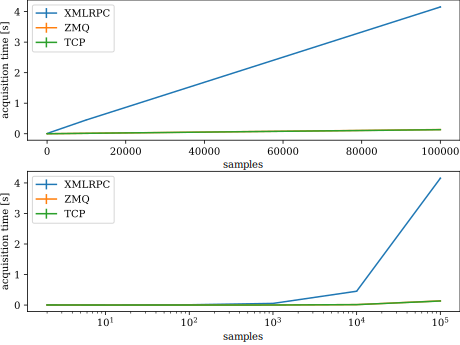
\includegraphics[width=\textwidth]{figures/measurements/xml_zmq_tcp_comparison_pickle.pdf}
            	\caption{Comparison of the acquisition speed using XMLRPC, ZeroMQ and TCP}
                \label{fig:meas:xml_zmq_tcp_comp_pikle}
            \end{minipage}
            \vfill
            \vspace{1cm}
            \begin{minipage}[b]{0.8\textwidth}
                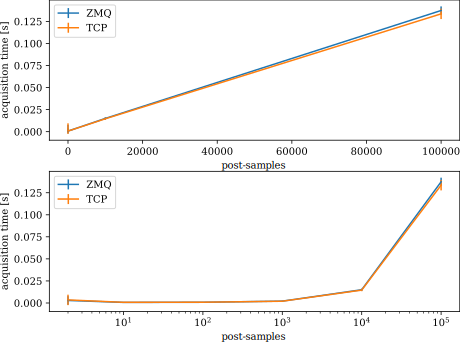
\includegraphics[width=\textwidth]{figures/measurements/zmq_tcp_comparison_pickle.pdf}
            	\caption{Comparison of the acquisition speed using ZeroMQ and TCP}
                \label{fig:meas:zmq_tcp_comp_pikle}
            \end{minipage}
        \end{figure}
        
        As the next step, three serialisation methods were compared (the serialisation libraries are described in section~\ref{subsec:serialisation}):
        \begin{itemize}
            \item Pickle,
            \item JSON,
            \item Protocol Buffers.
        \end{itemize}
        
        The measurements were done using both kinds of sockets: ZeroMQ and TCP. The results are presented in Fig. \ref{fig:meas:ser_comp_zmq} and Fig. \ref{fig:meas:ser_comp_tcp}.
        
        \begin{figure}
            \centering
            \begin{minipage}[b]{0.8\textwidth}
            	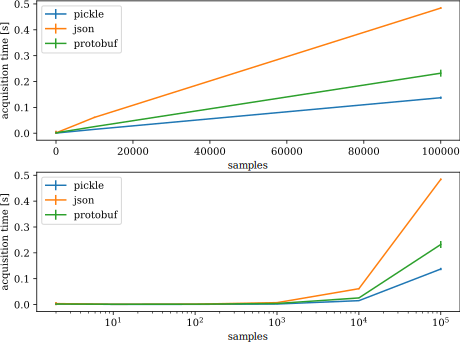
\includegraphics[width=\textwidth]{figures/measurements/zmq_serialization_comp.pdf}
            	\caption{Comparison of the serialisation libraries using ZeroMQ}
            	\label{fig:meas:ser_comp_zmq}
            \end{minipage}
            \vfill
            \vspace{1cm}
            \begin{minipage}[b]{0.8\textwidth}
            	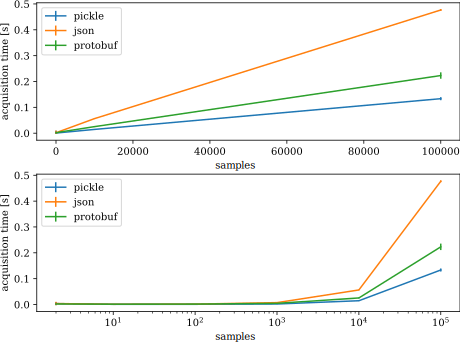
\includegraphics[width=\textwidth]{figures/measurements/tcp_serialization_comp.pdf}
            	\caption{Comparison of the serialisation libraries using TCP}
            	\label{fig:meas:ser_comp_tcp}
            \end{minipage}
        \end{figure}

        Clearly, in both cases the best result are obtained using Pickle as the serialisation library, therefore this library is used for all of the following measurements.
         
        Since the results obtained using ZeroMQ and TCP are very similar, even though TCP has slightly better performance, it ZeroMQ is used in the project, in order not to introduce too many technologies and for being consistent with the technology used for the RPC. The added value of the performance's increase would not be enough to compensate for the complication of the project.
        
        While optimising the acquisition loop, presented in the following section, another part of the code was also optimised. The acquired raw data had to be converted to volts. Before, each sample was converted in the standard Python loop. Since this part of code was introducing big delays, the Numpy \cite{numpy} library was used to convert the data. This optimisation resulted in significant increase of the acquisition speed. In order to be able to compare the following optimisation with previous results, the measurements were repeated, with the optimised convertion method. Otherwise, it would not be clear if the increase in performance was caused by a different conversion method or by acquisition speed optimisation. Moreover, it was desired to make sure that with this optimisation, there still would not be a great difference between the ZeroMQ and the TCP. The results are presented in Fig.~\ref{fig:meas:zmq_tcp_comp_pikle_numpy}. 
        
        \begin{figure}
        	\centerline{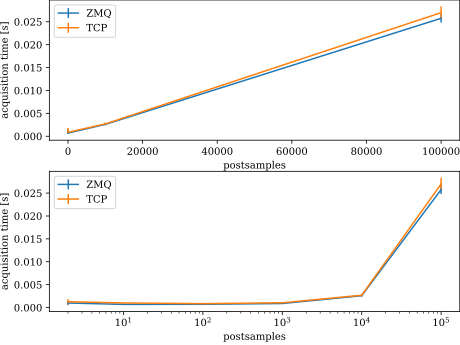
\includegraphics[width=0.8\textwidth]{figures/measurements/zmq_tcp_comparison_pickle_numpy.pdf}}
        	\caption{Comparison of the acquisition speed using ZeroMQ and TCP after code optimisations}
            	\label{fig:meas:zmq_tcp_comp_pikle_numpy}
        \end{figure}
        
        The increase of the acquisition speed when compared to the previous results was significant. However, the difference between the ZeroMQ and the TCP remained small. Therefore, all other measurements were performed using ZeroMQ sockets.
        
    \subsection{Optimisation of the acquisition loop} \label{section:acquisition_loop_opt}
        In the first approach,  when the DO Server was receiving a command to start a continuous acquisition from a particular GUI, it was configuring all the necessary ADCs to start a single acquisition. The ADC with a master configuration (see~section~\ref{section:data_synchronisation}) was configured at the and to make sure that the WRTD timestamps would be distributed only after all the other ADCs were already configured. The DO Server, after receiving the data from all required ADCs, was processing the data and sending it to the GUI. After that, the procedure was repeated. In this approach, the acquisition loop was situated in the DO Server.
        
        In the second approach, when the DO Server is receiving a command to start a continuous acquisition from a particular GUI, it is configuring the ADCs to start a continuous acquisition. The received data from all of the ADCs is buffered. After receiving the data from all the required ADCs, with corresponding timestamps, the data is sent to the GUI. In this approach, the acquisition loop is situated in the ADC.
        
        The simplified DO Server's state machines diagrams for both approaches are presented in Fig.~\ref{fig:loop_server_fsm} and Fig.~\ref{fig:loop_adc_fsm}.
        
        \begin{figure}
            \centering
            \begin{minipage}[b]{0.45\textwidth}
            	\includegraphics[width=\textwidth]{figures/loop_server_fsm.pdf}
            	\caption{The simplified state machine in the DO Server --- the acquisition loop in the DO Server}
                \label{fig:loop_server_fsm}
            \end{minipage}
            \hfill
            \begin{minipage}[b]{0.45\textwidth}
            	\includegraphics[width=\textwidth]{figures/loop_adc_fsm.pdf}
            	\caption{The simplified state machine in the DO Server --- the acquisition loop in the ADC}
                \label{fig:loop_adc_fsm}
            \end{minipage}

        \end{figure}
        
        The first approach was easier to implement, since it was much easier to debug. The ease of debugging was caused by the following reasons:
        \begin{itemize}
            \item The timestamps were distributed only after all of the ADCs were already configured. Therefore, the issues caused by trying to trigger a not configured ADC did not have to be taken into account.
            \item The successive data would not arrive into the DO Server before the previous one was already processed. Therefore, any errors could be immediately detected. When the problem occurred, the DO Server application was not flooded with the consecutive data. Moreover, when the DO Server was processing the data too slow it was not causing any error --- the only effect was that the acquisition frequency was getting lower.
        \end{itemize}
        
        Even though the approach with the acquisition loop in the DO Server was easier to implement, it was decided to move the acquisition loop to the ADC, since a significant increase in the performance was expected.
        
        In order to compare the performance of both approaches, the acquisition frequency for various numbers of pre-samples was measured. The configuration of the boards was exactly the same as the one described in section~\ref{section:data_transport_opt}.
        
        The acquisition frequency was calculated based on the number of data packets received from from the DO Server, during 0.5~s, calculated from the moment of sending the request to start a continuous acquisition. Each measurement was repeated 5 times. The results are presented in Fig. \ref{fig:meas:loop_adc_server_comp}. The plots represent the medium value, the vertical lines the standard deviation. 
        
        \begin{figure}
        	\centerline{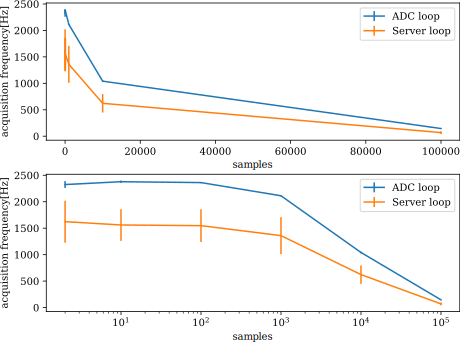
\includegraphics[width=0.8\textwidth]{figures/measurements/loop_adc_server_comparison.pdf}}
        	\caption{Comparison of the acquisition frequency when the acquisition loop is placed in the DO Server and in the ADC}
            	\label{fig:meas:loop_adc_server_comp}
        \end{figure}
        
        From the presented measurements it is clear that the optimisation of the acquisition loop increased the performance of the system significantly. It is worth noting, that the approach with the acquisition loop in the DO Server has much bigger variance. It is caused by the fact that in this approach the frequency depends on a bigger number of factors --- more commands are exchanged between the DO Server and the ADC. Therefore, there is a greater probability that a latency in the communication channel would occur.
        
\section{Measurements of the precision of the synchronisation} \label{section:precision_measurements}
    When acquiring the data synchronously, one of the most important parameters is the precision of the data synchronisation. In the DO the precision depends on the precision of timestamping of the acquired signal and on the precision of the timestamping clock. The timestamping clock is the WR clock, whose accuracy is of 1~ns (section \ref{section:WR}). Taking into account the fact that the timestamping clock (period 8~ns) is not locked to the sampling clock (10~ns period), the precision of the timestamping is of 10~ns. Therefore, the expected precision of the data synchronisation is of 11~ns.
    Another factor that has to be taken into account is that, because of ongoing modification of the hardware development conventions, there is no access to the EEPROM chip which stores the calibration data of the ADC, therefore the used ADCs are not calibrated.
    
    The signals are provided to the ADCs over 8~ns cables. However, the precision of the cables measurement is not known. In order to identify the errors introduced by the cables, all the precision measurements are repeated, switching the cables.
    
    The precision of the DO was measured using the setup presented in section \ref{section:hardware_setup}.
    The accuracy is measured as a distance of the zero-crosses between the measured signals from the two ADCs. The precision is calculated as 3$\sigma$ value of the normal distribution fitted to the measured data. The first ADC is triggered internally, the other by the timestamp from the previous one. The zero-cross is defined as a value for which a linear function is zero. The linear function is defined by two points: the last point whose value is negative and the first point whose value is positive. The measured signal was a square wave of frequency 1~kHz.
    
    The distance was measured 20000 times. The histograms of the measurements are presented in Fig. \ref{fig:meas:wrtd} and in Fig. \ref{fig:meas:wrtd_sig_rev}.
    
    \begin{figure}
        \centering
        \begin{minipage}[b]{0.8\textwidth}
        	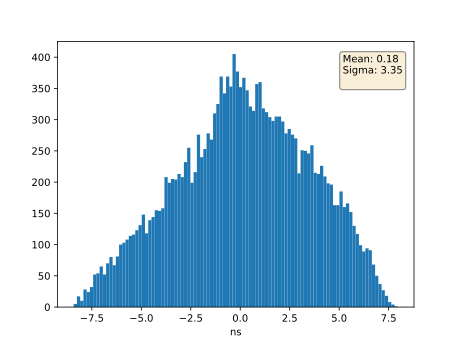
\includegraphics[width=\textwidth]{figures/measurements/WRTD.pdf}
        	\caption{The histogram of the accuracy of the data synchronisation.}
            \label{fig:meas:wrtd}
        \end{minipage}
        \vfill
        \vspace{0.5cm}
        \begin{minipage}[b]{0.8\textwidth}
        	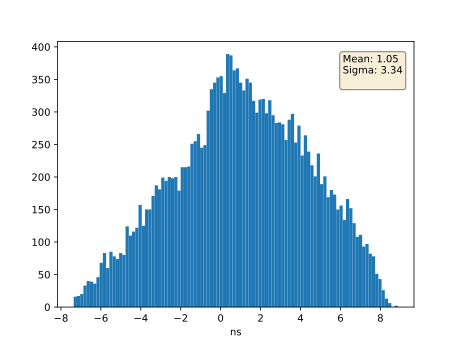
\includegraphics[width=\textwidth]{figures/measurements/WRTD_sig_rev.pdf}
        	\caption{The histogram of the accuracy of the data synchronisation, cables reversed.}
            \label{fig:meas:wrtd_sig_rev}
        \end{minipage}
    \end{figure}
    
    
    The results are very close to the expected ones: the mean value is equal 0.18~ns in the first configuration of the cables and 1.05~ns in the second configuration. Therefore, the difference between the cables lengths, measured in time of the signal propagation, is $ (1.05\:ns - 0.18\:ns)/2 = 0.44\:ns$. 
    As a proof that the lack of calibration could be the result of the mean value different from 0, the measurement was repeated, with the offset of the signal optimised to minimise the absolute value of the distance between the zero-crosses. The results are presented in Fig. \ref{fig:meas:wrtd_calib}. The shape of the distribution remains the same, only the mean value is moved to zero. 
    
    \begin{figure}
    	\centerline{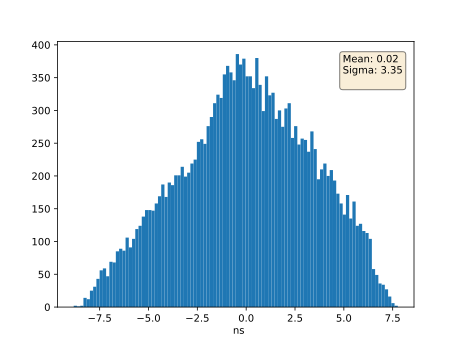
\includegraphics[width=0.8\textwidth]{figures/measurements/WRTD_calibration.pdf}}
        	\caption{The histogram of the accuracy of the data synchronisation, offset optimised.}
            \label{fig:meas:wrtd_calib}
    \end{figure}
    
    The value of 3$\sigma$ is equal to 10~ns. This result is slightly better than the expected one of 11~ns. 


    However, it must be stated, that the mean of the distribution can vary with time. Fig. \ref{fig:meas:wrtd_other_day} presents the same measurements taken another day. 
    \begin{figure}
    	\centerline{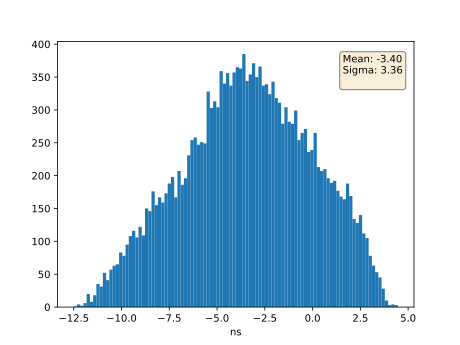
\includegraphics[width=0.8\textwidth]{figures/measurements/WRTD_other_day.pdf}}
        	\caption{The histogram of the accuracy of the data synchronisation taken another day.}
            \label{fig:meas:wrtd_other_day}
    \end{figure}
    The histogram shape remains the same, however the mean value is different. This behaviour could be partially caused by temperature differences of the board, which could explain differences in the range of few hundreds pico-seconds. Other sources of such behaviour should be investigated in the future work.